\chapter{Accounts \small{\textsf{DRAFT}}}\label{chapter.accounts}

In our treatment so far, we have dealt with the UTXO model. There, the state
that we maintained was the UTXO set, and transactions expressed a \emph{transition}
from one UTXO set to the next by updating it appropriately (adding and removing elements from
it). By ordering the transactions into a ledger using a blockchain, we achieved
consensus on a mutually shared state between mistrustful participants, among
which an honest majority assumption holds. The machinery
we have created solves the \emph{State Machine Replication}\index{State Machine Replication}
problem.

However, the machinery that we used to achieve consensus, namely the block and the chain,
was quite separate from the semantic interpretation of the transactions that are confirmed
in the produced ledgers. During the block validation process, we asked the full nodes
to validate transactions by ensuring that the UTXO set can appropriately transition
from one state to the next.

Certain aspects of the validation concern the \emph{consensus layer}\index{Consensus Layer},
which pertains to checking the consensus contents of blocks: The ancestry relation,
the genesis block, the proof-of-work, the timestamps, the difficulty adjustment mechanism.
These checks pertain to the \emph{structural validation} of blocks.

\begin{figure}[h]
  \centering
  \includegraphics[width=\columnwidth,keepaspectratio]{figures/tx-state-transition.pdf}
  \caption{Transitioning state by applying transactions.}
  \label{fig.state-transition}
\end{figure}

\section{Accounts Model}

\subsection{Accounts Model Compared with UTXO Model}
Recall the previous UTXO model: we store a set of unspent transaction outputs (UTXOs). When a transaction occurs, UTXOs corresponding to the transaction's inputs are removed and UTXOs corresponding to the transaction's outputs are added into the UTXO set to produce a new UTXO set, as shown in Figure \ref{fig.UTXOModelDiagram}.

\begin{figure}[h]
    \centering
    \begin{tikzpicture}[
    squarednode/.style={rectangle, draw=black, thick, auto},
    ]

    \node[squarednode]   (state0)                               {UTXO Set};
    \node[align=center]             [below=0.2cm of state0]     {State 0};
    \node[squarednode]   (state1)   [right=3cm of state0]       {UTXO Set};
    \node[align=center]             [below=0.2cm of state1]     {State 1};
    \node[squarednode]   (state2)   [right=3cm of state1]       {UTXO Set};
    \node[align=center]             [below=0.2cm of state2]     {State 2};

    \draw[->, black, thick]     (state0) -- node[midway,above] {tx} (state1);
    \draw[->, black, thick]     (state1) -- node[midway,above] {tx} (state2);

    \end{tikzpicture}
    \caption{State transitions in the UTXO model}
    \label{fig.UTXOModelDiagram}
\end{figure}

The accounts model is another model of transactions.
% Transactions in the UTXO model consume previous outputs and generate new outputs. However, i
In the accounts model, transactions contain 1) the account that sends balance (from), 2) the account that receives balance (to), 3) the value of the transaction (val), 4) the transaction fee (fee), and 5) the signature on the transaction ($\sigma$).

\begin{figure}[h]
\centering
    \begin{tabular}{|c|c|c|c|c|}
         \hline
         From & To & Val & Fee & {$\sigma$} \\
         \hline
    \end{tabular}
    \label{fig.accountsTx}
    \caption{Structure of a transaction in the accounts model}
\end{figure}

For the accounts model, the state is maintained by accounts (public keys) and balances, as shown in Figure \ref{fig.AccountsModelDiagram} and Figure \ref{fig.balanceState}.

\begin{figure}[h]
    \centering
    \begin{tikzpicture}[
    squarednode/.style={rectangle, draw=black, thick, auto},
    ]

    \node[squarednode]   (state0)                               {Balances};
    \node[align=center]             [below=0.2cm of state0]     {State 0};
    \node[squarednode]   (state1)   [right=3cm of state0]       {Balances};
    \node[align=center]             [below=0.2cm of state1]     {State 1};
    \node[squarednode]   (state2)   [right=3cm of state1]       {Balances};
    \node[align=center]             [below=0.2cm of state2]     {State 2};

    \draw[->, black, thick]     (state0) -- node[midway,above] {tx} (state1);
    \draw[->, black, thick]     (state1) -- node[midway,above] {tx} (state2);

    \end{tikzpicture}
    \caption{State transitions in the accounts model}
    \label{fig.AccountsModelDiagram}
\end{figure}

\begin{figure}[ht]
    \centering
        \begin{tabular}{c|c}
        \multicolumn{2}{c}{Balances State} \\
        \hline
        Alice   & 5 bu  \\
        \hline
        Bob     & 100 bu \\
        \hline
        Dionysis & 1 bu \\
        \hline
        \end{tabular}
    \caption{Balance State}
    \label{fig.balanceState}
\end{figure}

The function that takes in a state and a transaction and returns a new state is called a \textbf{transition function}. It has a general form of:

\begin{equation}
    \delta (st,tx) =
        \begin{cases}
        st' & \text{if $tx$ valid w.r.t. $st$} \\
        \perp & \text{otherwise} \\
        \end{cases}
\end{equation}

Specifically, the transition function of UTXO model is given by:

\begin{equation}
    \delta_{UTXO} (st,tx) =
        \begin{cases}
        st \setminus tx_{in} \cup tx_{out}  & \text{if $tx$ valid w.r.t. $st$} \\
        \perp & \text{otherwise} \\
        \end{cases}
\end{equation}

Where $tx_{in}$ is the set of unspent outputs in the ``inputs'' field of $tx$, and $tx_{out}$ is the set of newly generated outputs in the ``outputs'' field of $tx$.

The transaction validation process of UTXO model is
\begin{itemize}
    \item[-] Check $\sigma$
    \item[-] Check conservation
    \item[-] Check inputs are in $st$
\end{itemize}

Similarly, the transition function of the accounts model could be written as:

\begin{equation}
    \delta_{acc} (st,tx) =
        \begin{cases}
        st' & \parbox[t]{.6\textwidth}{where $st' [tx.from] = st [tx.from] - tx.value$, \\
        $st' [tx.to] = st [tx.to] + tx.value$, if $tx$ valid w.r.t. $st$} \\
        \perp & \text{otherwise} \\
        \end{cases}
\end{equation}

The transaction validation process of the accounts model is
\begin{itemize}
    \item[-] Check $\sigma$
    \item[-] Check $st [tx.from] \geq tx.value$
\end{itemize}

\subsection{Accounts Model Replay Attack}

Here comes a problem. In the accounts model, if the same transaction is sent to the network twice, should the second transaction be included or not? For example, one morning, Bob bought a cup of coffee from Starbucks. The next morning, he bought a cup of coffee again. These two transactions have the same fields, even the signature.

If the network decides to accept transactions that are the same, the following replay attack could happen: an adversarial coffee shop could replay the transaction even if Bob didn't buy a coffee. However, if the network decided not to include transactions that are same, then Bob could only buy a coffee once.

The solution is to add a nonce field to transactions. The nonce is an 256-bit integer per source account which is incremented every new transaction. The transaction structure now looks like Figure \ref{fig.accountsTxWithNonce}.

\begin{figure}[ht]
\centering
    \begin{tabular}{|c|c|c|c|c|c|}
         \hline
         From & To & Val & Fee & \textbf{nonce} & {$\sigma$} \\
         \hline
    \end{tabular}
    \caption{Structure of tx in accounts model}
    \label{fig.accountsTxWithNonce}
\end{figure}

And therefore, while validating transactions, an additional step of validating the nonce should be included. Transactions in which the nonce
has already been used is rejected.
% and all other fields are the same are only included once.
This means that the state contains the current nonce for each account, in addition to the balance.
The state transition function must also update the nonce for the ``from'' account of the transaction.

A side by side comparison between the two models  of transactions is shown in Figure \ref{fig.sideBySide}.

\begin{figure}[ht]
    \centering
    \begin{tabular}{m{3cm}|m{4cm}|m{6.5cm}}
         & UTXO & Accounts  \\
         \hline
         Real System & Bitcoin & Ethereum \\
         \hline
         Transaction $tx$ & 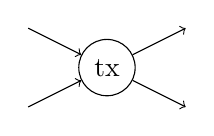
\begin{tikzpicture}[
         txnode/.style={thin,draw=black,circle},
         ]
         \node[txnode] (tx) at (0,0) {tx};
         \draw[->] (-1,0.5) -- (tx);
         \draw[->] (-1,-0.5) -- (tx);
         \draw[->] (tx) -- (1, 0.5);
         \draw[->] (tx) -- (1,-0.5);
         \end{tikzpicture}
         &
         \begin{tabular}{|c|c|c|c|c|c|}
         \hline
         From & To & Val & Fee & \textbf{nonce} & {$\sigma$} \\
         \hline
         \end{tabular} \\
         \hline
         Transistion $\delta$ & {Remove consumed outputs and add produced outputs} & \makecell{Update balances \\ $st'[from] \coloneqq st[from] - value$ \\ $st'[to] \coloneqq st[to] + value$} \\
         \hline
         Validation & {Signature, Law of Conservation, Inputs exist in $st$.} & {Signature, Sufficient balance, Nonce unique.} \\
         \hline
         Genesis State & $\emptyset$ & $\{\}$ \\
         \hline
    \end{tabular}
    \caption{Side by Side Comparison of Two Models}
    \label{fig.sideBySide}
\end{figure}

\section{State Machine Replication}
We talk briefly about State Machine Replication (SMR).
A state machine consists of a state, inputs and a transition function. The machine has an initial state. Based on its inputs and the state transition function, the machine updates its state.
In SMR, multiple nodes in the network run a state machine in a distributed manner.
The term ``replication'' signifies that each node in the network maintains the state of the machine and runs its transition functions locally.
The goal of SMR is that each node runs the same set of state transitions and in the same order so that there is agreement or consensus on the state of the machine.

A blockchain can be considered as a distributed replicated database. A blockchain can help us run SMR. We have seen two examples of state machines that the blockchain can run --- the accounts model and the UTXO model. In both cases, there is a state $st$, state transition functions $\delta$, and inputs (which are transactions in this case). The initial state is specified by the genesis state.

\section{Light Clients}

How to run a blockchain node efficiently? Efficiency has multiple dimensions: storage, communication, and computation. For most application scenarios, the blockchain node has limited resources. For example, if we store all the data of the chain, it would take gigabytes of storage. Validating every transaction in the network would be very heavy work for a phone. Therefore, a light client is needed for these resource-limited nodes.

\subsection{Storage Efficiency: Merkle Trees}

For a light client, it is better to save the data at a server and retrieve data at usage. However, we need to prove the integrity of the retrieved data. Hash functions are useful in this case. Suppose that we wanted to store a file on a server and verify that we receive the correct file from the server. We could hash the file and store the hash (checksum) locally. When we request files from the data server, we validate the checksum of the retrieved file to verify that it is the exact file we saved on the server. However, this requires clients to retrieve the entire file to validate its integrity even if only a 1 kilobyte chunk is needed.

We can also split the file into chunks and hash each chunk. This reduces the communication complexity: clients only need the chunk to be transferred. However, this requires more hash key storage for the client. The client needs to store one hash per chunk, making the storage complexity linear in the size of the file. There is a trade off between communication complexity and storage complexity: with large chunks, comes high communication complexity and with small chunks, comes high storage complexity.

Our goal is to achieve low storage and low communication. Specifically, storage with $O(1)$ complexity and communication with $O(\log n)$ complexity where $n$ is the number of chunks of the file. And this is done with a data structure called Merkle tree.

\subsection{Data Structure: Merkle Tree}

Files are split into $n$ data chunks.
$$
D: D[0], D[1], ..., D[n-1]
$$

A binary tree of depth $\mu$ is created, where there are $2^\mu = n$ leaves (for simplicity, assume that $n$ is a power of 2). Each node in the binary tree stores a hash $h$ which is the hash of its children concatenated.
$$
h \coloneqq H(h[\mathrm{left}] \mathbin\Vert h[\mathrm{right}])
$$

Nodes on the leaves store the hash of the corresponding data chunk. The client stores the Merkle tree root (MTR) $h_\epsilon$. When a data chunk is requested, the server sends the data chunk, along with every sibling hash value to the clients as shown in Figure \ref{fig.merkleTree}. For example, when data chunk at index $j$ is requested, the server sends $D[j]$, $\pi_0$, $\pi_1$, $\pi_2$, and $\pi_3$ to the client. The client walks from the received data chunk all the way up to the root to check if the hash values are intact. From calculating $e_0$ by hashing the data chunk, to the top level $e_{\mu+1}$, the client calculates $e_k = H(e_{k-1} \mathbin\Vert \pi_{k-1})$ or $e_k = H(\pi_{k-1} \mathbin\Vert e_{k-1})$(left child first). In this example, the client computes the values $e_0 = H(D[j])$, $e_1 = H(e_0 \mathbin\Vert \pi_0)$, $e_2 = H(\pi_1 \mathbin\Vert e_1)$, $e_3 = H(e_2 \mathbin\Vert \pi_2)$, and $e_4 = H(\pi_3 \mathbin\Vert e_3)$ and then compares $e_4$ with $h_\epsilon$.

\begin{figure}[ht]
    \centering
    \begin{tikzpicture}[grow=down,sloped,
    level distance=1.5cm,
    level 1/.style={sibling distance=6cm},
    level 2/.style={sibling distance=4cm},
    level 3/.style={sibling distance=2.5cm},
    level 4/.style={sibling distance=1.5cm},]
    \node {$h_\epsilon$}
     child {
        node {$\pi_3$}
        child {
            node {$H(...)$}
            child {
                node {$H(H(D[0]) \mathbin\Vert H(D[1]))$}
                child {
                    node {$H(D[0])$}
                    node[below=5mm] {$D[0]$}
                }
                child {
                    node {$H(D[1])$}
                    node[below=5mm] {$D[0]$}
                }
            }
            child {
                node {$...$}
            }
        }
        child {
            node {$...$}
        }
     }
     child {
        node {$e_3$}
        child {
            node {$e_2$}
            child {
                node {$\pi_1$}
                child {
                    node {$...$}
                }
                child {
                    node {$...$}
                }
            }
            child {
                node {$e_1$}
                child {
                    node {$e_0$}
                    node[below=5mm] {$D[j]$}
                }
                child {
                    node {$\pi_0$}
                    node[below=5mm] {$...$}
                }
            }
        }
        child {
            node {$\pi_2$}
            child {
                node {$...$}
            }
            child {
                node {$H(...)$}
                child {
                    node {$...$}
                }
                child {
                    node {$H(D[n-1])$}
                    node[below=5mm] {$D[n-1]$}
                }
            }
        }
     }
     node[below=2mm] {$e_4$}
     ;

    \end{tikzpicture}
    \caption{Merkle Tree}
    \label{fig.merkleTree}
\end{figure}

With this data structure, the data transferred is a list of $\pi$ values and the data chunk of fixed size, which gives $\lvert \pi \rvert = O(\log n)$ succinct communication and $O(1)$ constant storage.

The Merkle tree structure is described by the functions
\begin{align}
\mathrm{compress}(D) &\rightarrow h_\epsilon,\\ \mathrm{prove}(D, j) &\rightarrow \pi, \text{ and} \\ \mathrm{verify}(h_\epsilon, d, j, \pi) &\rightarrow \begin{cases}
\mathrm{true} & \text{if valid} \\
\mathrm{false} & \text{otherwise}
\end{cases}.
\end{align}
The correctness of the Merkle tree is specified as:
\begin{align}
    \forall D, \forall j,
    \mathrm{verify}(\mathrm{compress}(D), D[j], j, \mathrm{prove}(D, j)) = \mathrm{true}
\end{align}

\subsection{Security of Merkle Trees}

MT-security means that if the client outputs true after verifying the received data chunk and proof, then the received data must be the same data that was originally stored.
To define security of Merkle trees formally, we create the following game that lets an adversary try to break the protocol.

\begin{center}
    \begin{lstlisting}[mathescape=true]
$\mathrm{MERKLE}_{\mathcal{A}}(\kappa)$:
    $D,\pi,j,d$ $\leftarrow$ $\mathcal{A}(1^\kappa)$
    return $\mathrm{verify}(\mathrm{compress}(D), d, j, \pi) \land d \neq D[j]$
    \end{lstlisting}
\end{center}

Our goal is to prove that

$$
\forall \text{ PPT } \mathcal{A}: Pr[\mathrm{MERKLE}_{\mathcal{A}}(\kappa) = 1] \leq negl(\kappa)
$$
\begin{theorem}
Let $H$ be a collision-resistant hash function. Then Merkle trees constructed with H are MT-secure.
\end{theorem}

\begin{proof}
Suppose for contradiction, $\mathcal{A}$ breaks MT-security. We will construct an adversary $\mathcal{A}'$ that breaks collision-resistance of $H$.

\begin{center}
    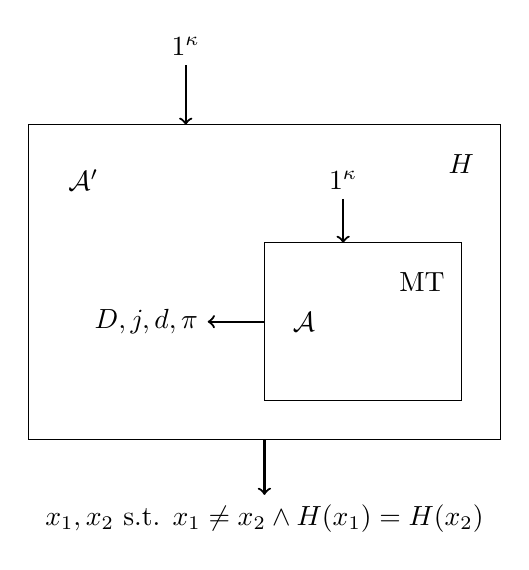
\begin{tikzpicture}
        \draw[draw=black] (0,0) rectangle (6, -4);
        \draw[draw=black] (3,-1.5) rectangle (5.5, -3.5);

        \node at (3.5,-2.5) {$\mathcal{A}$};
        \node at (5,-2) {MT};

        \node at (0.7,-0.7) {$\mathcal{A}'$};
        \node at (5.5,-0.5) {$H$};

        \node (inner_input) at (4,-0.7) {$1^\kappa$};
        \node (inner_output) at (1.5,-2.5) {$D, j, d, \pi$};

        \node (input) at (2,1) {$1^\kappa$};
        \node (output) at (3,-5) {$x_1, x_2$ s.t. $x_1 \neq x_2 \land H(x_1) = H(x_2)$};

        \draw[->, thick] (3,-2.5) -- (inner_output);
        \draw[->, thick] (inner_input) -- (4,-1.5);

        \draw[->, thick] (input) -- (2,0);
        \draw[->, thick] (3,-4) -- (output);
    \end{tikzpicture}
\end{center}

We use $e$ for the hash value calculated by the client, $h$ for the expected hash value in the correct Merkle tree, and $\pi$ for the hash values returned by the server.

Consider the event that $\mathcal{A}$ succeeds, i.e. $\mathrm{verify}(\mathrm{compress}(D), d, j, \pi) = 1 \land d \neq D[j]$.

$\mathcal{A}'$ works as follows:

Given that $\mathcal{A}$ succeeds, the returned list of $\pi$ is used to calculate hashes of the nodes to verify the returned data chunk, which involves calculating $e$ values by concatenating the children of the nodes. The hash of the root is the same ($h_\epsilon = e_{top}$)
and the hash of the data chunk is different ($e_0 \neq h_0$). (If not, $\mathcal{A}'$ has already found a collision because different data chinks have the same hash.)
Therefore, there must exist a node, some level $k$ in the tree, such that $e_k = h_k$ but its children $e_{k-1}$ or $\pi_{k-1}$ not equal to the expected $h$ values. (These must exist because roots are the same, but leaves are different). In this case, we have two different inputs that hash to the same value.

Then, adversary $\mathcal{A}'$ returns children of $e_k$ from the verifier tree at level $k$ as $x_1$ and children of $h_k$ from real tree at the corresponding position as $x_2$. Then, $x_1$ and $x_2$ satisfy $x_1 \neq x_2 \land H(x_1) = H(x_2)$.

Therefore, the probability of breaking the Merkle tree protocol is the same as the probability of breaking the collision-resistant hash function $H$.
$$
Pr[\mathrm{MERKLE}_{\mathcal{A}}(\kappa) = 1] = Pr[\mathrm{Collision}_{\mathcal{A}'}(\kappa) = 1]
$$

But $Pr[\mathrm{Collision}_{\mathcal{A}'}(\kappa) = 1]$ is negligible by assumption, which means the probability of breaking Merkle tree protocol is also negligible.

\end{proof}
